\documentclass[11pt,a4paper]{article}

\usepackage[margin=20mm,landscape]{geometry}
\usepackage{amsmath,amssymb}
\usepackage{graphicx}
\usepackage{booktabs}
\usepackage{array}
\usepackage{xcolor}
\usepackage{microtype}
\usepackage[colorlinks=true,linkcolor=blue!55!black,urlcolor=blue!55!black]{hyperref}

\definecolor{ink}{HTML}{0B0B0B}
\definecolor{soft}{HTML}{52514E}
\definecolor{accent}{HTML}{2A78D6}
\definecolor{warn}{HTML}{D03B3B}

\newcommand{\Lsym}{L_{\mathrm{sym}}}
\newcommand{\note}[1]{{\color{soft}\small #1}}

\graphicspath{{wp2024_picked/}{wp2033_picked/}}

% A portrait map on the left, a short caption on the right.
\newcommand{\mapslide}[2]{%
  \noindent
  \begin{minipage}[c]{0.62\linewidth}\centering
    \includegraphics[width=\linewidth,height=0.86\textheight,keepaspectratio]{#1}
  \end{minipage}\hfill
  \begin{minipage}[c]{0.34\linewidth}
    #2
  \end{minipage}}

% Two portrait maps side by side.
\newcommand{\twomaps}[2]{%
  \noindent
  \begin{minipage}[t]{0.49\linewidth}\centering
    \includegraphics[width=\linewidth,height=0.80\textheight,keepaspectratio]{#1}
  \end{minipage}\hfill
  \begin{minipage}[t]{0.49\linewidth}\centering
    \includegraphics[width=\linewidth,height=0.80\textheight,keepaspectratio]{#2}
  \end{minipage}}

\title{\textbf{Spectral Clustering of the Irish Transmission Grid}\\[2mm]
\large Where the grid comes apart}
\author{Oleksandr \quad---\quad Team 6, Electrical Grid Hackathon 2026}
\date{Networks: \texttt{WP2024} and \texttt{WP2033}, all-island}

\begin{document}
\maketitle

% ---------------------------------------------------------------------------
\vspace{8mm}
\noindent
\begin{minipage}[t]{0.52\linewidth}
\textbf{Method}
\begin{enumerate}\itemsep2pt
  \item Grid as a weighted graph: buses and generators are nodes.
  \item Normalised Laplacian $\Lsym = I - D^{-1/2} A\, D^{-1/2}$.
  \item Its $k$ smallest eigenvectors as coordinates per node.
  \item $k$-means on those coordinates.
\end{enumerate}
\end{minipage}\hfill
\begin{minipage}[t]{0.44\linewidth}
\textbf{Edge weights}

\medskip
\begin{tabular}{@{}ll@{}}
\toprule
susceptance & $1/x_e$ --- static network\\
headroom    & $s_{\text{nom}} - |F_e|$ --- one hour of dispatch\\
\bottomrule
\end{tabular}

Spectral clustering could help in bottle necks finding. Although analysis here is taken for two different weight, 
they are not fully independent of each other. 

First, "susceptance" is an inverse of reactance so higher reactance - lower the weight. 
This agreeds with electric flow, so the higher weight, the more probable for a flow to choose this route.

Second, "headroom" is an absolute value of power that is still possible to put in the line. 
Note that this weight is load dependent.

Based on weights and the way of clusering the resulting clustering is expected to find a bootle necks 
and hence this method could help in identification of the congested lines. 
For this purpose, a DC aproximation of electric flow is used to find the actual the most loaded lines.
\end{minipage}

% ---------------------------------------------------------------------------
\newpage
\section*{WP2024 --- where the grid is loaded}

\mapslide{congested_lines_WP2024_all-island_lf0.5_capped}{This is a heated map 
of the grid with simulated results of currnt flow via PyPsa. It is used for 
reference for a clustering.%
Branches at $\ge 50\%$ of rating over one week.

\medskip
57 of 848 branches.}

% ---------------------------------------------------------------------------
\newpage
\section*{WP2024 --- clustering, \texorpdfstring{$k=6$}{k=6}: headroom and susceptance}

\twomaps{clusters_sym_headroom_k6_20300120_1700}{clusters_sym_susceptance_k6}
These clusters looks in someway similar and could actually find the problematic part. Hovewer, some of congested lines are remaining hidden for any type of spectral clustering. 

% ---------------------------------------------------------------------------
\newpage
\section*{WP2024 --- the north-east cluster}

\mapslide{cluster_4}{%
171 nodes, linked to the rest through a few corridors. The transformator or/and 
line near it were found found as corridors on each spectral clustering performed. 
It also agreeds with electric flow simulation. }


% ---------------------------------------------------------------------------
\newpage
\section*{WP2024 --- the week: how close the grid is to splitting}

\begin{center}
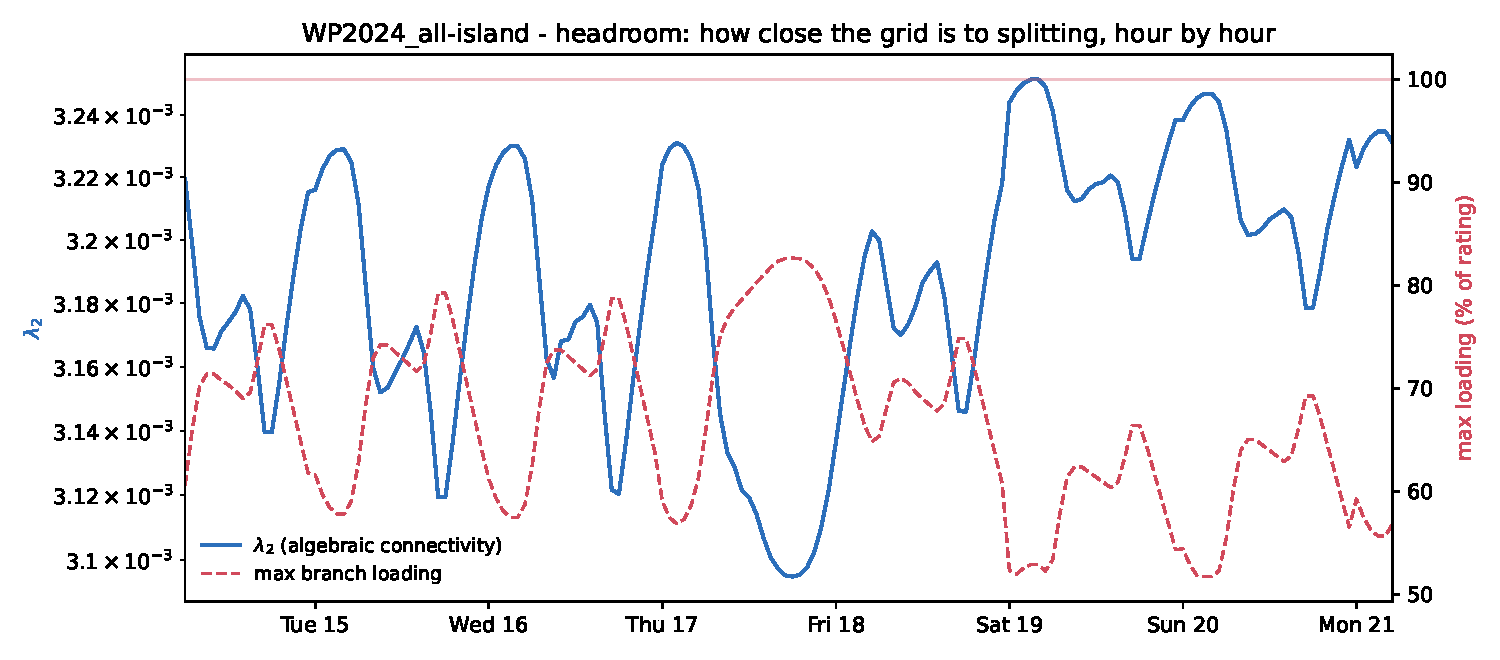
\includegraphics[width=\linewidth,height=0.78\textheight,keepaspectratio]{lambda2_sym_headroom}
\end{center}

\noindent
As the spectral clustering is already used for one of the flow simulations, the next question follows naturally. 
Does clustering patttern changes over the week?
$\lambda_2$ dips whenever the maximum branch loading peaks. 

% ---------------------------------------------------------------------------
\newpage
\section*{WP2024 --- the week: does the partition move?}

\begin{center}
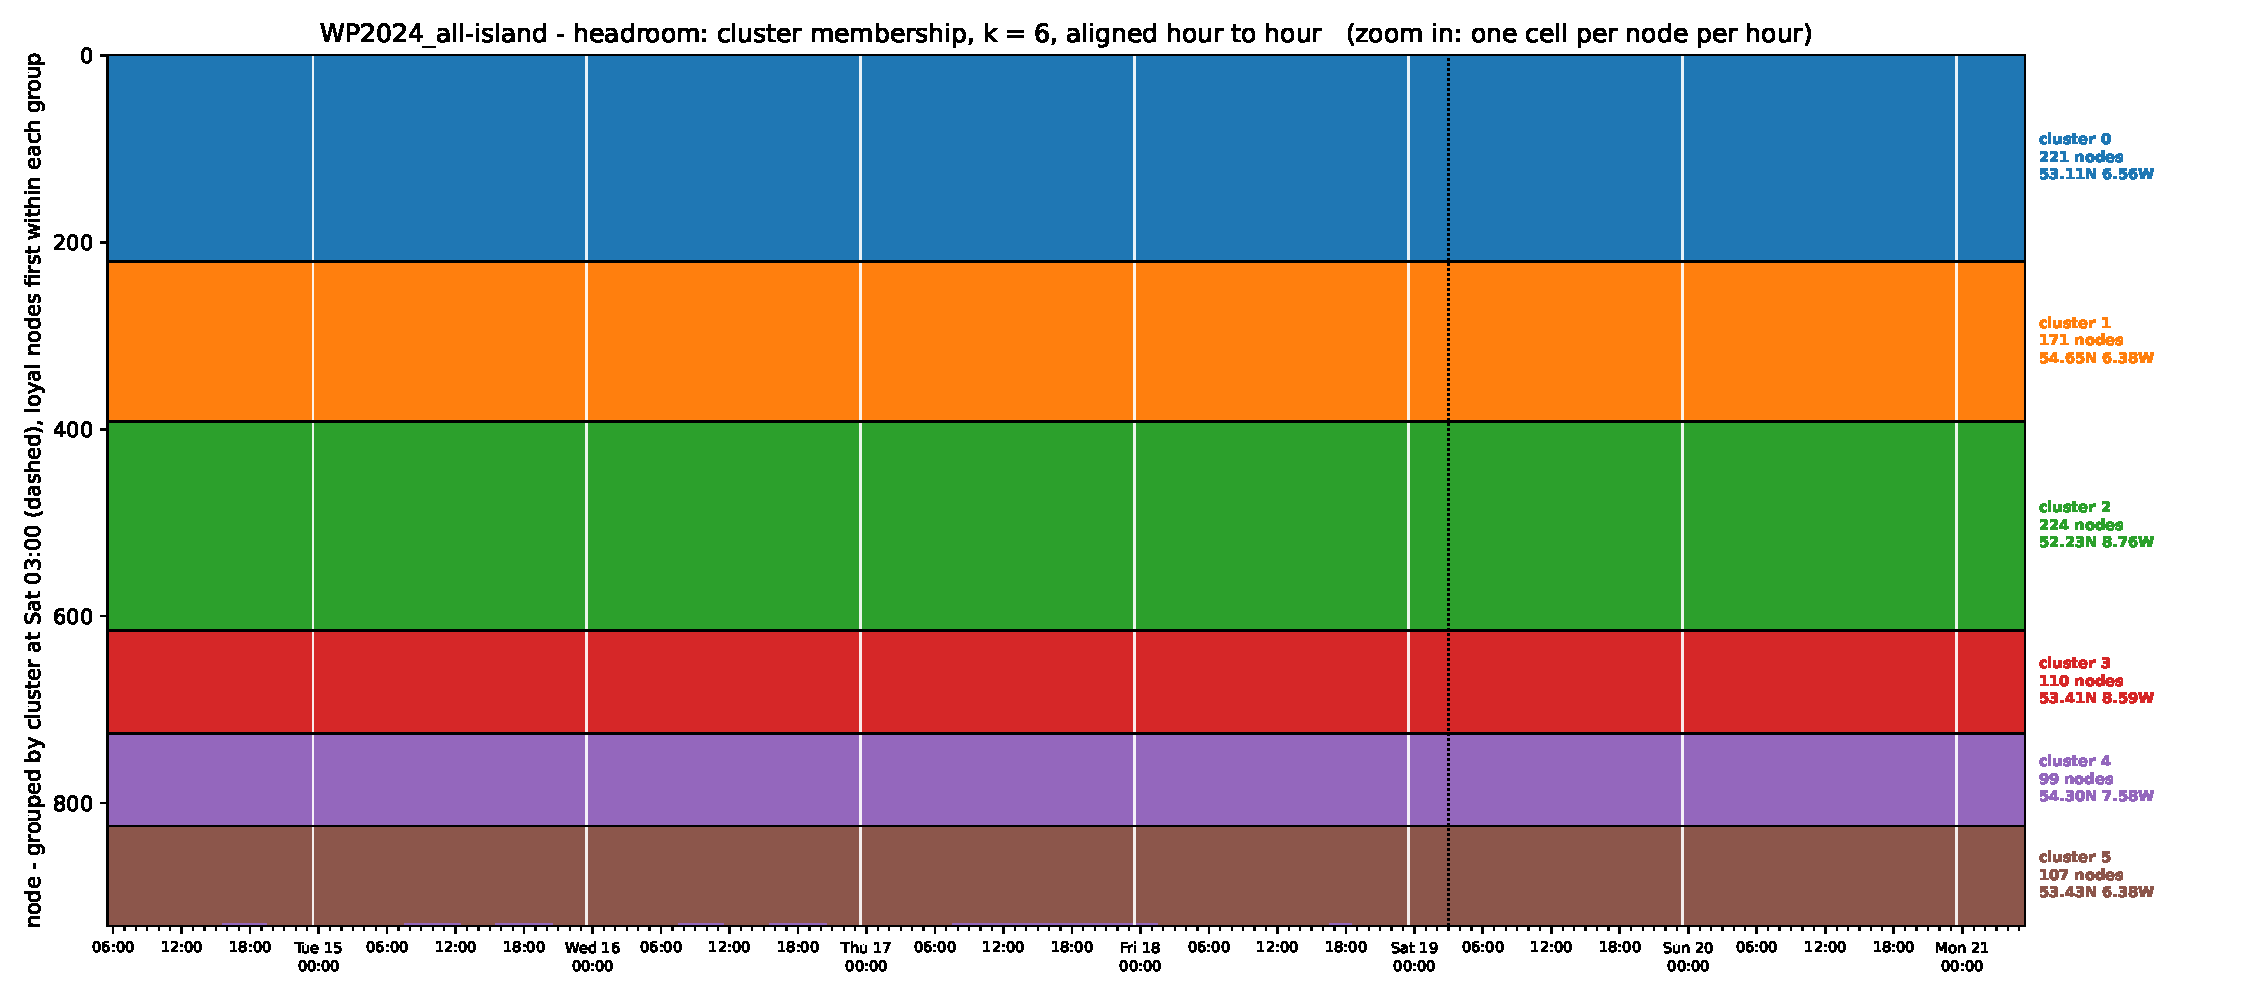
\includegraphics[width=\linewidth,height=0.78\textheight,keepaspectratio]{membership_sym_headroom_k6}
\end{center}

\noindent
No node changes cluster over the 168 hours, 
which suggest that the network topology 
has more effect on the spectering then loading for non extreme cases.

% ---------------------------------------------------------------------------
\newpage
\section*{WP2024 --- the eigenvalues: how many clusters?}

\begin{center}
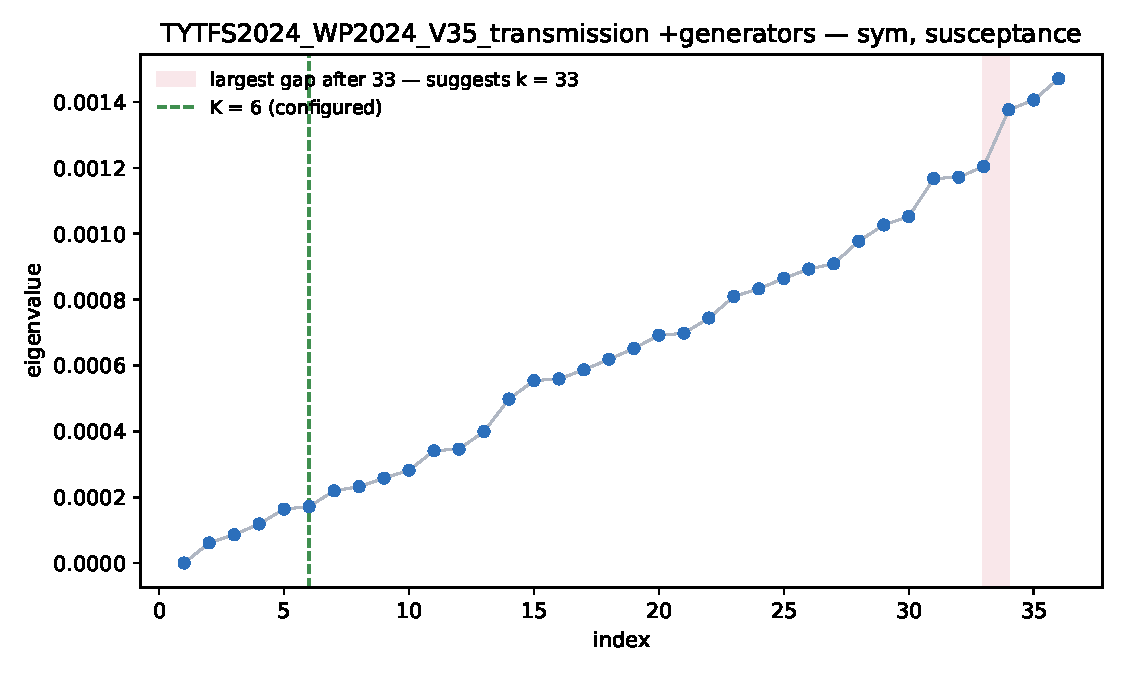
\includegraphics[width=\linewidth,height=0.78\textheight,keepaspectratio]{spectrum_sym_susceptance}
\end{center}

\noindent
A note on the number of clusters. To find the best number of clusters, the eigen gaps are calculated. 
It is clear that some of the clusters are prefered to another. Hovewer, the best eigen gap is after 33.
So it motivates to check clustering with $k=33$.

% ---------------------------------------------------------------------------
\newpage
\section*{WP2024 --- susceptance clustering, \texorpdfstring{$k=33$}{k=33}}

\mapslide{clusters_sym_susceptance_k33}{%
As this is already seen, this graph is a total mess. Unfortunately, no hidden patterns or similarity to congested lines were found.}

% ---------------------------------------------------------------------------
\newpage
\section*{WP2033 --- where the grid is loaded}

\mapslide{congested_lines_WP2033_all-island_lf0.7_capped}{%
The previous analysis was applied to the stable grid, but what is more unstable (the predicted one) is taken?
Branches at $\ge 70\%$ of rating over one week.

\medskip
66 of 980 branches.}

% ---------------------------------------------------------------------------
\newpage
\section*{WP2033 --- clustering, \texorpdfstring{$k=6$}{k=6}: headroom and susceptance}

\twomaps{wp2033_picked/clusters_sym_headroom_k6_20300120_1700}{wp2033_picked/clusters_sym_susceptance_k6}

Same problems and same ideas are applied to this case. The clustering doesn't improove. No new patters are found.

Hence, the conclusion is that electric network works much different from the traffic or water flow and identification of bottle necks doesn't give a full picture. 
The improovement to this method is to account for an electricity effects and consider something else on top of pure topology. Alternatively, 
use some other metric to assing values (for each generator) and then classify them in clusters.
% ---------------------------------------------------------------------------
\newpage
\section*{WP2033 --- generators grouped by sensetivity, \texorpdfstring{$k=9$}{k=9}}

\mapslide{WP2033/generator_clusters_WP2033_k9}{%
$k$-means on each generator's sensetivity across 
all 980 branches. So this clustering technically 
shows how generators are similar between themself. 
The pattern here is relatively similar to the above analysis, 
which agreeds with the fact that some of the congested lines 
were identified as bottle neck (so topology of network is important parameter 
but definitly not the only one)}

% ---------------------------------------------------------------------------
\newpage
\thispagestyle{empty}
\vspace*{\fill}
\begin{center}
\resizebox{0.6\linewidth}{!}{\textbf{NEXT}}
\end{center}
\vspace*{\fill}

% ---------------------------------------------------------------------------
% Full-page background figure, "Questions?" on top. A4 landscape is
% 842 x 595 pt; the picture origin sits one \topskip (11 pt) below the top.
\newpage
\newgeometry{margin=0mm}
\thispagestyle{empty}
\setlength{\unitlength}{1pt}
\noindent
\begin{picture}(0,0)
  \put(0,-584){\makebox(842,595){%
    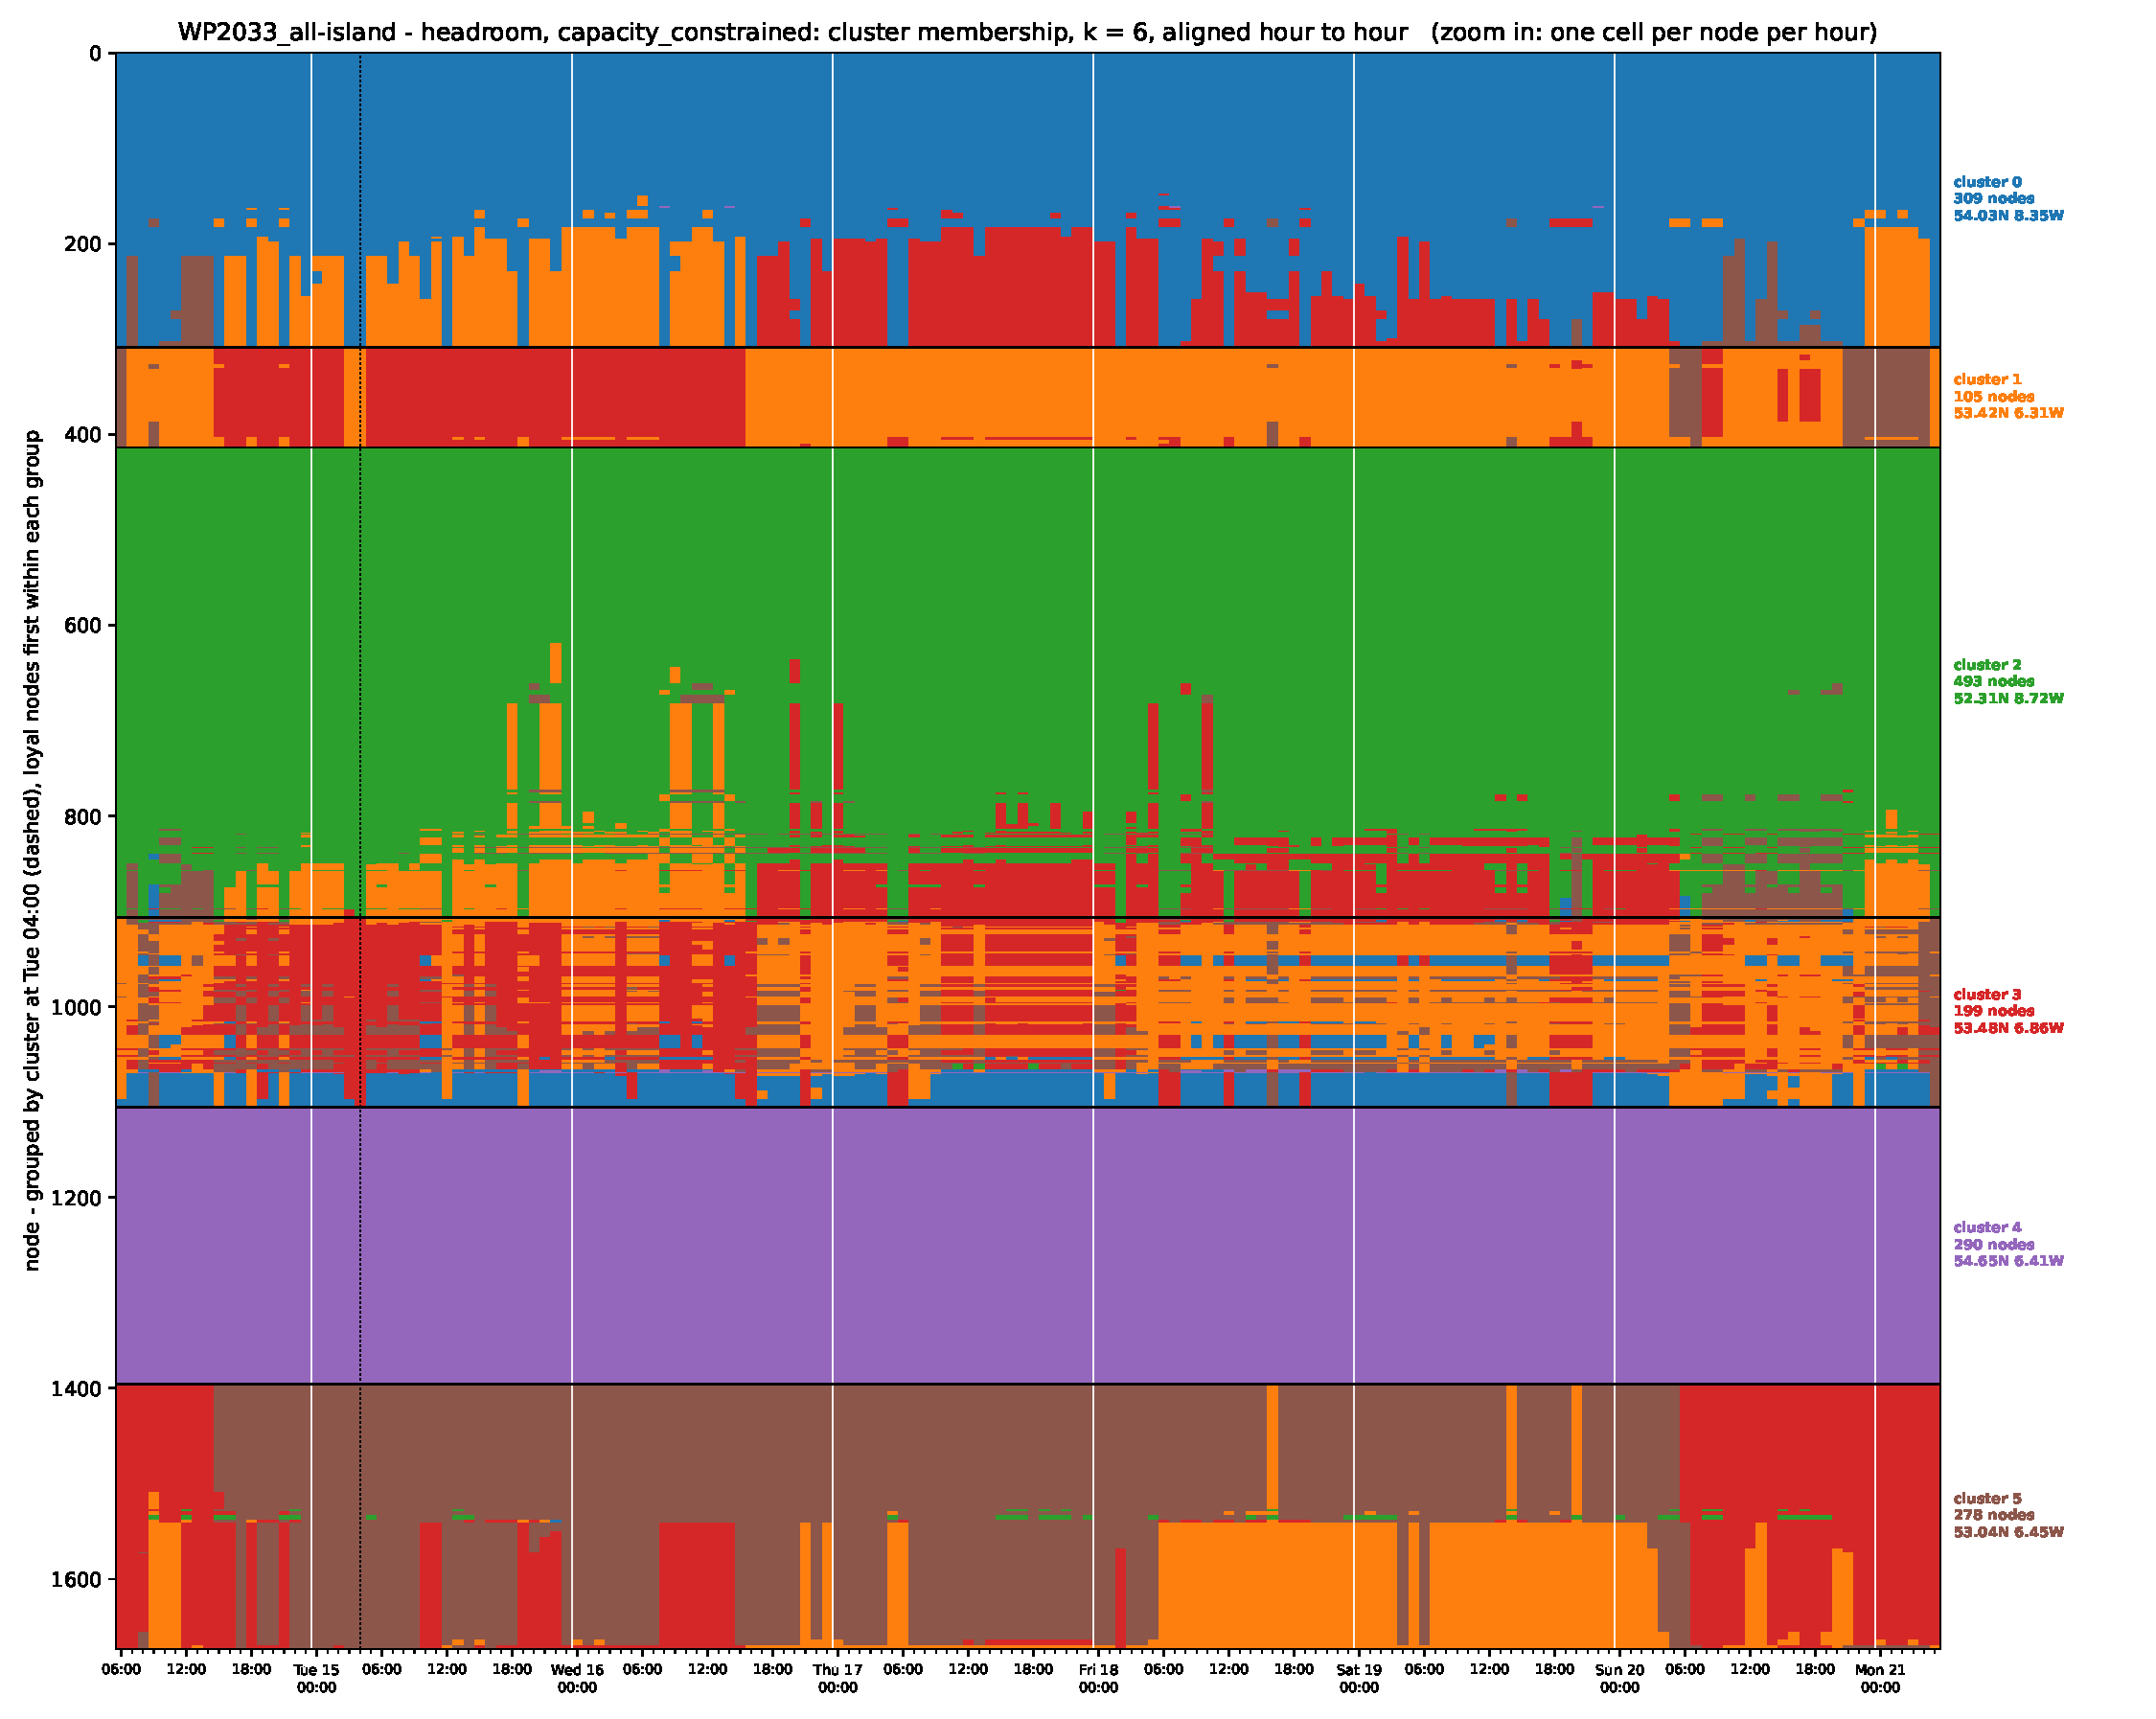
\includegraphics[width=842pt,height=595pt,keepaspectratio]{WP2033/membership_sym_headroom_capped_k6}}}
  \put(0,-600){\makebox(842,595){%
    \colorbox{white}{\resizebox{0.45\paperwidth}{!}{\textbf{Questions?}}}}}
\end{picture}

\end{document}
